%%%%%%%%%%%%%%%%%%%%%%%%%%%%%%%%%%%%%%%%%%%%%%%%%%%%%%%%%%%%%%%%%%%%%%%%
%                                                                      %
%     File: Thesis_Kinematics_Dynamics                                 %
%     Tex Master: Thesis.tex                                           %
%                                                                      %
%     Author: Francisco Castro                                         %
%     Last modified :  16 Jan 2024                                      %
%                                                                      %
%%%%%%%%%%%%%%%%%%%%%%%%%%%%%%%%%%%%%%%%%%%%%%%%%%%%%%%%%%%%%%%%%%%%%%%%

\chapter{Proposed Approach}
\label{chapter:proposedApproach}

%	A partir do problem statement da introdução e com base na revisão do estado da arte, apresenta-se a formulação do problema numa forma matemática. A partir da revisão do estado da arte estabelecida anteriormente, descreve-se aqui a abordagem escolhida para a implementação de cada um dos módulos, assim como a metodologia de interação entre os mesmos. Por outro lado, também é apresentada informação que será repetida ao longo da tese na forma de funções, por forma que não existam repetições desnecessárias.

\section{Problem formulation}
\label{section:problemFormulation}

The problem laid out in this thesis is to yield a Nonlinear Model Predictive Control (\acrshort{nmpc}) \cite{rawlings:MPC, grune:NMPC} algorithm $\mathbb{P}$, which models the kinematics and dynamics of a rigid wheeled, autonomous robot $\mathcal{R}$ as well as its interactions with the terrain during the traversal of a semi-unknown, off-the-road, uneven terrain map $\mathcal{M} \subset \mathbb{R}^3$, resembling a planetary environment. It is required that the robot avoids untraversable areas or obstacles $\mathcal{\ObstacleSpace} \subset \mathcal{\Map}$, and follows a time optimal traversable pathway to reach a goal point $\mathnormal{G} \in \mathcal{M}$, starting from a given initial admissable pose $\mathcal{R}_p \in \Map \setminus \mathcal{\ObstacleSpace}$. Moreover, the robot $\mathcal{R}$ shall make a fast, safe and slippage-free traverse, as well as minimizing the energy consumed by the robot battery.  The algorithm $\mathbb{P}$ must be computationally optimal and update the system actuation in a timely fashion.

\section{Optimal path planning}
\label{section:optimalPathPlanning}

\subsection{Cost map generation}
\label{subsection:costMapGen}

This thesis is mainly focused on \acrlong{nmpc}, so a simple approach to yield a suitable traversability map is chosen. Both the elevation, $\ElevationMap$,  and traversability, $\TraversabilityMap$, maps are assumed to be known \ti{a-priori} and will be computed off-line.

\begin{assumption}
	The elevation and traversability maps are assumed to be known \ti{a-priori} without uncertainties, resembling the fact that planetary terrains are scanned \ti{prior} to the placement of a rover on the ground.
	\label{assumption:frames}
\end{assumption}

Due to its compactness and simplicity, \acrlong{dem} are chosen to describe the elevation $\Elevation$ at each location $(x_i, y_j)$. Then, from the compacted data, a cost map approach is followed in order to yield a traversability map  of the environment, by assigining a traversability cost $\TraversabilityCost$ to each grid point $(x_i, y_j)$. This choice stems from the fact that this is a popular trend in the planetary robotics literature, but also because it is easily combined with a minimum-cost planner algorithm, in order to output a global planner. Finally, the elevation and traversability maps can be joined in a two-layered map $\TwoLayerMap$, because boths domains are equal. Morever, these frames are considered to share the same frame $\WorldFrame$, because both map frames match at the origin. An algorithm to address this plan is presented in section \ref{section:costMap}. It is built on top of the works of \citet{Amorim2014} and \citet{Ishigami2007PathPlanning} and provides \textcolor{red}{complete subsection by linking map generation to path planning algorithm and by adding short description of the implementation}.

\section{Mobile robot kinematics}
\label{section:overview}

Kinematics describe the motion geometry of a point or body according to the provided actuations. A four-wheeled rover-like kinematics model is to be derived in this chapter, which can be applied both to skid-steering or differentially driven mobile robots.

A wheeled mobile robot $\Robot$ is moving on a map $\Map$, which is centered at the origin of an inertial frame $\WorldFrame$. A moving frame $\BodyFrame$ is centered on the robot's center of mass \acrshort{com} and it is fixed to $\Robot$. Although the mobile robot operates on unstructured, uneven, off-the-road terrains, not all \acrshort{dof} are controllable. This issue is addressed in the following sections.

\begin{assumption}
	In moving frame $\BodyFrame$, $\BodyFrame_x$ points forward, $\BodyFrame_y$ points to the left and $\BodyFrame_z$ points upwards. Regarding world frame $\WorldFrame$, its axis directions are dictated by ROS' standard axis directions \cite{Foote2010}.
	\label{assumption:frames}
\end{assumption}

\begin{figure}[!htb]
  	\centering
  	\subfigure[Robot moving frame]{
    		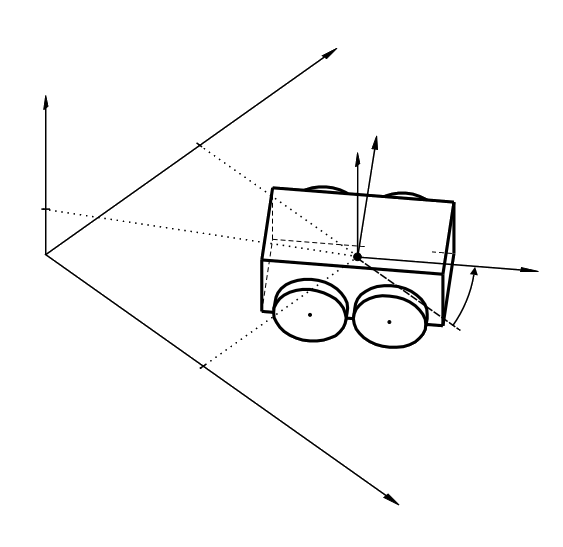
\includegraphics[width=0.25\linewidth]{Figures/robotMovingFrame.png}
    }\hfill
    \subfigure[Robot geometry]{
    		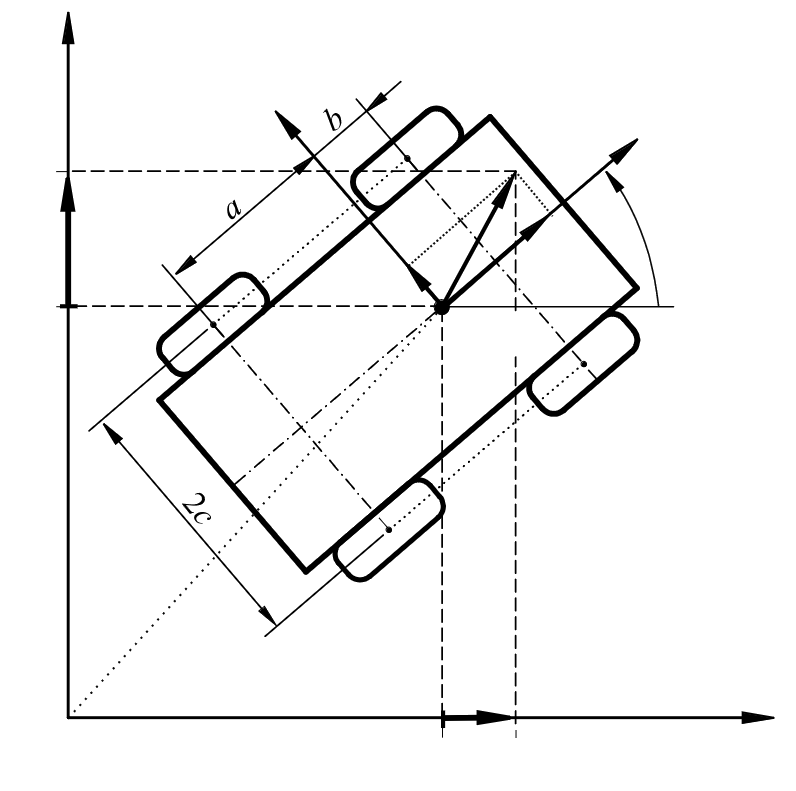
\includegraphics[width=0.32\linewidth]{Figures/robotGeometry.png}
    	}\hfill
    \subfigure[ICR]{
    		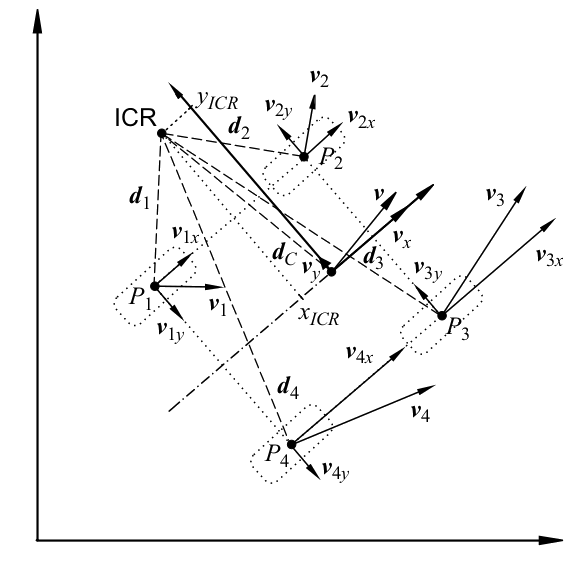
\includegraphics[width=0.32\linewidth]{Figures/ICR.png}
  	}
  	\caption{Car-like robot kinematics \cite{Kozlowski2004}}
	\label{fig:mobileRobotKinematics}
\end{figure}

The mobile robot position and orientation with respect to frame $\WorldFrame$ is described as $\mathbf{\Position} = [x\;  y\; z]^T$ and $\Quaternion = [\qx \; \qy \; \qz \; \qw]^T$, respectively. On the other hand, the mobile robot linear and angular velocities with respect to frame $\BodyFrame$ stands as $\mathbf{\LinVelocity} = [ \vx \; \vy \; \vz ]^T$ and $\bm{\AngVelocity} = [\wx \; \wy \; \wz]^T$, respectively. It is decided to use quaternions instead of euler angles to describe the orientation, in order to circumvent ambiguities  present on the sum of angles. Moreover, due to the fact that the yaw angle is constrained in $[-\pi,\,\pi]$, there is a chance that the yaw angle may overcome these limits when the mobile robot is close to them. \textcolor{red}{add section where more information will be given on the issues of euler angles ambiguities}.  Then, it is possible to map the mobile robot $\Robot$ linear velocity between frames $\BodyFrame$ and $\WorldFrame$ by taking advantage of rotation matrix \ref{eq:quatRotationMatrix}, but also to map quaternion rates in $\WorldFrame$ to angular velocities in $\BodyFrame$ with rotation matrix \ref{eq:orientationQuatRotationMatrix}.

\begin{minipage}{0.4\linewidth}
	\centering	
	\begin{equation}
	\DerMathBold{\Position} = \mathbf{\RotMatrix}_{\BodyFrame}^{\WorldFrame} \mathbf{\LinVelocity}	
	\label{eq:translationFreeBody}
	\end{equation}
\end{minipage}
\begin{minipage}{0.4\linewidth}
	\centering	
	\begin{equation}
	\DerMathBold{\Quaternion} = \mathbf{\bar{\RotMatrix}}_{\BodyFrame}^{\WorldFrame} \bm{\AngVelocity}	
	\label{eq:rotationFreeBody}
	\end{equation}
\end{minipage}

\subsection{Wheel kinematics}
\label{subsection:wheelKinematics}

A kinematics model is not only described by its free-body motion equations \ref{eq:translationFreeBody} and \ref{eq:rotationFreeBody}, but also by geometrical constraints \cite{Kozlowski2004}. Each wheel is actuated by a torque $\Torque_i$, which induces on it a spin rate, $\bm{\AngVelocity}_i,\, i = 1,\,...,\,N_w$, where $N_w = 4$ for the cases presented in this thesis. 

\begin{assumption}
	The thickness and deformation of each wheel are neglected so that the wheel is assumed to be rigid and to contact the terrain at a single contact point $\contactPoint_i$, in case rigid terrain is the working environment \cite{Iagnemma2004}.
	\label{assumption:singlePointContact}
\end{assumption}

Due to the fact that wheels are fixed, the mobile robot holds two controllable \acrshort{dof}: translation along its longitudinal direction $\BodyFrame_x$, and rotation around its vertical axis $\BodyFrame_z$. Therefore, lateral skidding from the vehicle is expected to remain close to zero on flat terrain, although its wheels are prone to skidding when the mobile robot finds itself on uneven or inclined surfaces (figure \ref{fig:wheelForcesMoments}). If the mobile robot follows a straight line path, its wheel velocities are tangent to the current path. Moreover, the velocity vector of each wheel is tangent to the terrain that wheel is touching on.

The terrain profile imposes $\wx$ and $\wy$. On the other hand, the existence of holes or bumps force $\vz$ to be different from zero. $\vy$ rises above zero in case of lateral skidding.

If a mobile robot is not following a straight line path, this robot will rotate around an \acrshort{icr} point. Each wheel angular velocity is equal to the mobile robot angular velocity, $\bm{\AngVelocity}$. The vector $\mathbf{\positionVector}_i$, which connects the ICR point to each wheel position, is orthogonal to each wheel velocity $\mathbf{\LinVelocity}_i = [ \vx \; \vy \; \vz ]^T_i$, as well as $\mathbf{\positionVector}_C \perp \mathbf{\LinVelocity}$, so the following relations may be derived by taking into account the general expression $\mathbf{\LinVelocity} = \bm{\AngVelocity} \times \mathbf{r}$. Vectors $\mathbf{\LinVelocity}_i$, $\mathbf{\positionVector}_i$, $\mathbf{\positionVector}_C$ and $\mathbf{\wheelPosition}_i$ are all expressed with respect to frame $\BodyFrame$.

\begin{equation}
	\begin{cases}
		\vx = \wy d_{C, z} - \wz d_{C, y} \quad \vx_i = \wy d_{i, z} - \wz d_{i, y}\\
		\vy = \wz d_{C, x} - \wx d_{C, z} \quad \vy_i = \wz d_{i, x} - \wx d_{i, z}\\
		\vz = \wx d_{C, y} - \wy d_{C, x} \quad \vz_i = \wx d_{i, y} - \wy d_{i, x}
	\end{cases}
	\label{eq:3dICR}
\end{equation}

Then, it is possible to relate $\mathbf{\positionVector}_C$ to $\mathbf{\positionVector}_i$, with $\mathbf{\positionVector}_C = \mathbf{\positionVector}_i + \mathbf{\wheelPosition}_i$, where $\mathbf{\wheelPosition}_i$ is a vector which connects each wheel center's position to the moving frame origin. If this relationship is introduced into equation \ref{eq:3dICR}, it comes that,

\begin{equation}
	\mathbf{\LinVelocity}_i = \mathbf{\LinVelocity} + \bm{\omega} \times \mathbf{\wheelPosition}_i
	\label{eq:wheelVel}
\end{equation}

From the analysis of the previous equation, it is possible to state that,

\begin{equation}
	\begin{aligned} 
	\begin{cases}
		\vx_1 = \vx_2 \\
		\vx_3 = \vx_4 
	\end{cases}
	\end{aligned}, \qquad
	\begin{aligned}
		\begin{cases}
			\vy_1 = \vy_4 \\
			\vy_2 = \vy_3 
		\end{cases}
	\end{aligned}, \qquad
	\begin{aligned}
		\begin{cases}
			\vz_3 - \vz_2 = ( \wheelPosition_{3, y} + \wheelPosition_{2, y} ) \wx \\
			\vz_4 - \vz_1 = ( \wheelPosition_{4, y} + \wheelPosition_{1, y} ) \wx \\
			\vz_2 - \vz_1 = ( \wheelPosition_{2, x} + \wheelPosition_{1, x} ) \wy \\
			\vz_3 - \vz_4 = ( \wheelPosition_{3, x} + \wheelPosition_{4, x} ) \wy \\
		\end{cases}
	\end{aligned}
	\label{eq:wheelKinematicConstraints}
\end{equation}

\subsection{Wheel-terrain contact angles}
\label{subsection:contactAngles}

In this thesis, it is important to retrieve each wheel's contact angle with the terrain it is touching on, in order to enable the transfer of forces applied at $\contactPoint_i$ to frame $\BodyFrame$ and to describe the velocity of each wheel with respect to a frame $\WheelFrame^i$ with axes $\WheelFrame^i_x$ and $\WheelFrame^i_y$ tangent to the terrain at $\contactPoint_i$. Apart from assumption \ref{assumption:frames} and \ref{assumption:singlePointContact}, this analysis takes two more assumptions into account:

\begin{assumption}
	Every wheel is touching the terrain at a point $\contactPoint_i$.
	\label{assumption:fullContact}
\end{assumption}

\begin{assumption}
	The velocity of each wheel is tangent to the terrain profile at $\contactPoint_i$.
	\label{assumption:velTangent}
\end{assumption}

Assumptions \ref{assumption:fullContact} and \ref{assumption:velTangent} ensure this analysis remains consistent with the fact that, without a contact point $\contactPoint_i$ between a wheel and the terrain, there would be no reason to obtain a contact angle or a wheel velocity tangent to the terrain.

At every wheel $i$, a frame $\WheelFrame^i$ is attached to the wheel center and follows up the wheel velocity vector at every time. The transformation from $\WheelFrame^i$ to $\BodyFrame$ is based on a rotation matrix expressed in equation \ref{eq:rotationMatrixB2T}. Frame $\WheelFrame^i$ cannot yaw with respect to $\BodyFrame$ because the wheels do not steer ($\yaw_i = 0$).

\begin{equation}
\mathbf{\RotMatrix}_{\WheelFrame^i}^{\BodyFrame} =
\begin{bmatrix}
 		\cos(\pitch_i) & \sin(\pitch_i) \sin(\roll_i) & \sin(\pitch_i) \cos(\roll_i) \\
 		0 & \cos(\roll_i) & -\sin(\roll_i) \\
 		-\sin(\pitch_i) & \cos(\pitch_i) \sin(\roll_i) & \cos(\pitch_i) \cos(\roll_i) \\
	\end{bmatrix}
	\label{eq:rotationMatrixB2T}
\end{equation}

, where $\pitch_i$ denotes the pitch component of the contact angle, whereas $\roll_i$ stands for the roll component of the contact angle. Finally, it is possible to express $\mathbf{\LinVelocity}_i$ with respect to frame $\WheelFrame^i$ (equation \ref{eq:wheelVelT}). This reasoning is depicted in figure \ref{fig:wheelKinematics}. 

\begin{equation}
	\mathbf{\LinVelocity}_i = \mathbf{\RotMatrix}_{\WheelFrame^i}^{\BodyFrame} \mathbf{\LinVelocity}_i^{\WheelFrame^i}
	\label{eq:wheelVelT}
\end{equation}

However, due to the fact the estimation of wheel contact angles involves the solution determination of a cumbersome system of equations \cite{IagnemmaDubowsy2004}. Moreover, if roll and pitch effect are both taken into account, this estimation becomes even more cumbersome. 

In this thesis, the state estimation problem is left aside, so the direction of $\WheelFrame^i$ is obtained by computing a vector $\mathbf{t}$, which is tangent to the surface of the elevation map $\FunctionElevation(\cdot)$ at $\contactPoint_i$, with coordinates $\left(\x_i,\,\y_i,\,\FunctionElevation\left( \x_i,\,\y_i \right) \right)$, which are ommited for the sake of brevity, from now on.

\begin{definition}
The directional derivative of a scalar function $f(x_1,\,\ldots, x_n)$ in the normalized direction $\mathbf{u} = \left(u_1,\,\ldots, u_n \right)$, denoted by $\nabla_{\mathbf{u}}f$, is defined to be $\nabla_{\mathbf{u}} f = \nabla f \cdot \mathbf{u}$.
\label{def:directionalDerivative}
\end{definition}

If the mobile robot longitudinal, forward bi-dimensional direction vector is $\mathbf{u} = \cos(\yaw) \mathbf{i} + \sin(\yaw) \mathbf{j}$, from the directional derivative definition (\ref{def:directionalDerivative}) it comes that $\nabla_{\mathbf{u}} \FunctionElevation = \nabla \FunctionElevation \cdot \mathbf{u} = \frac{\partial \FunctionElevation}{\partial \x} \cos(\yaw) + \frac{\partial \FunctionElevation}{\partial \y} \sin(\yaw)$. This result expresses the slope of the elevation map $\FunctionElevation\left(\cdot\right)$ at some point $\contactPoint_i \in \Map_2$ on the direction of $\mathbf{u}$, so $\mathbf{t_u} = [\cos(\yaw),\,\sin(\yaw),\,\nabla_{\mathbf{u}} \FunctionElevation]$. 

\begin{figure}[!h]
	\centering
	\subfigure[Longitudinal wheel kinematics.] {
		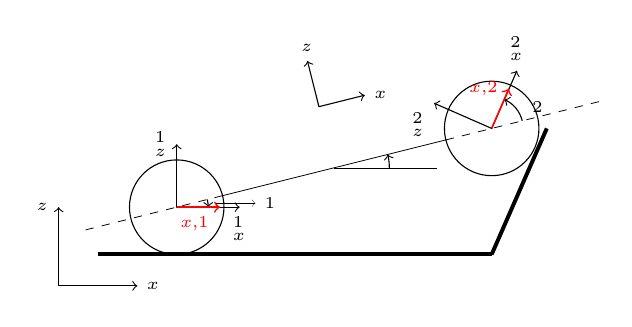
\begin{tikzpicture}
			%	Frames
			\draw[->] (0.5, 1) -- (1.5, 1) node[right] {\footnotesize $\WorldFrame_x$};
			\draw[->] (0.5, 1) -- (0.5, 2) node[left] {\footnotesize $\WorldFrame_z$};
			
			%	Circles			
			\draw (2.0, 2.0) circle (0.6cm);
			\draw (6.0, 3.0) circle (0.6cm);
			
			%	Circles center points			
			\fill (2.0, 2.0) circle (0.01cm);
			\fill (6.0, 3.0) circle (0.01cm);
			
			%	Linee between circles
			\draw[line width = 0.1mm] (2.582, 2.146) -- (5.418, 2.854);
			
			%	Body frame
			\draw[->] (3.806, 3.276) -- (4.388, 3.422) node[right] {\footnotesize $\BodyFrame_x$};
        		\draw[->] (3.806, 3.276) -- (3.660, 3.858) node[above] {\footnotesize $\BodyFrame_z$};
        		
        		%	Wheel frame 1
        		\draw[->] (2.0, 2.0) -- (2.8, 2.0) node[below] {\footnotesize $\WheelFrame_x^1$};
        		\draw[->] (2.0, 2.0) -- (2.0, 2.8) node[left] {\footnotesize $\WheelFrame_z^1$};
        		
        		%	Wheel frame 2
        		\draw[->] (6.0, 3.0) -- (6.3208, 3.7328) node[above] {\footnotesize $\WheelFrame_x^2$};
        		\draw[->] (6.0, 3.0) -- (5.2672, 3.3208) node[below left] {\footnotesize $\WheelFrame_z^2$};
        		\draw[line width = 0.5mm] (1.0, 1.4) -- (6.0, 1.4);
        		\draw[line width = 0.5mm] (6.0, 1.4) -- (6.7, 3.0);
        		\draw[line width = 0.1mm, dashed] (5.418, 2.854) -- (7.418, 3.354);
        		\draw[line width = 0.1mm, dashed] (2.582, 2.146) -- (0.8, 1.7);
        		\draw[line width = 0.05mm] (4.0, 2.5) -- (5.3, 2.5);
        		
			%	Arcs        		
        		\draw[->] (4.7, 2.5) arc [start angle=0, end angle=14.03624347, x radius = 0.7, y radius = 0.7] node[black, above right, pos=-0.5] {\footnotesize $\pitch$};
        		\draw[->] (2.388, 2.097) arc [start angle=14.03624347, end angle=0, x radius = 0.4, y radius = 0.4];
        		\draw[->, line width=0.1pt] (2.5, 2.05) -- (3.0, 2.05) node[right] {\footnotesize $\pitch_1$};
        		\draw[->] (6.388, 3.097) arc [start angle=14.03624347, end angle=66.357, x radius = 0.4, y radius = 0.4] node[black, above right, pos=-0.05] {\footnotesize $\pitch_2$};
        		
        		%	Velocity
        		\draw[->, line width = 0.2mm, red] (2.0, 2.0) -- (2.55, 2.0) node[red, below left] {\footnotesize $\LinVelocity_{x, 1}$};
        		\draw[->, line width = 0.2mm, red] (6.0, 3.0) -- (6.219, 3.505) node[red, left] {\footnotesize $\LinVelocity_{x, 2}$};
        		
		\end{tikzpicture}
	}
	\hfill
	\subfigure[Lateral wheel kinematics.] {
		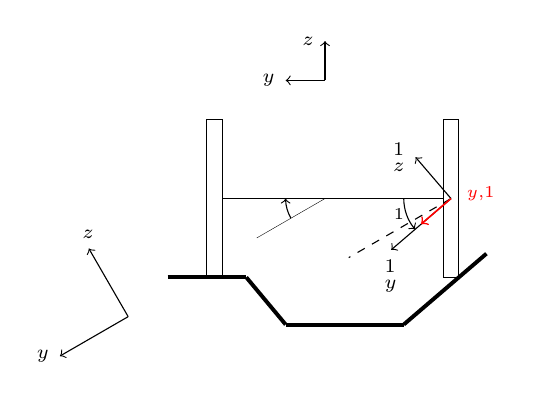
\begin{tikzpicture}
			%	World frame
			\draw[->] (0.0, 0.0) -- (-0.866, -0.5) node[left] {$\WorldFrame_y$};
			\draw[->] (0.0, 0.0) -- (-0.5, 0.866) node[above] {$\WorldFrame_z$};
			
			%	Body frame
			\draw[->] (2.5, 3.0) -- (2.0, 3.0) node[left] {$\BodyFrame_y$};
			\draw[->] (2.5, 3.0) -- (2.5, 3.5) node[left] {$\BodyFrame_z$};
			
			%	Wheel frame
			\draw[->] (4.1, 1.5) -- (3.341, 0.849) node[below] {$\WheelFrame_y^1$};
			\draw[->] (4.1, 1.5) -- (3.65, 2.025) node[left] {$\WheelFrame_z^1$};
			
			\draw[draw=black] (1.0, 0.5) rectangle ++(0.2, 2.0);
			\draw[draw=black] (4.0, 0.5) rectangle ++(0.2, 2.0);
			\draw[line width = 0.05mm] (2.5, 1.5) -- (1.634, 1.0);
			
			%	Arc
			\draw[->] (2.067, 1.25) arc [start angle=210, end angle=180, x radius = 0.5, y radius = 0.5] node[black, left, pos=0.2] {\footnotesize $\roll$};
			\draw[->] (3.5, 1.5) arc [start angle=180, end angle=220.601, x radius = 0.6, y radius = 0.6] node[black, above left] {\footnotesize $\roll_1$};
 			
			%	Line between wheels
			\draw[line width = 0.1mm] (1.2, 1.5) -- (4.0, 1.5);
			
			\draw[dashed] (4.1, 1.5) -- (2.801, 0.75);
			
			%	Terrain
			\draw[line width = 0.5mm] (0.5, 0.5) -- (1.5, 0.5);
			\draw[line width = 0.5mm] (1.5, 0.5) -- (2.0, -0.1);
			\draw[line width = 0.5mm] (2.0, -0.1) -- (3.5, -0.1);
			\draw[line width = 0.5mm] (3.5, -0.1) -- (4.55, 0.8);
			
			%	Velocity
        		\draw[->, line width = 0.2mm, red] (4.1, 1.5) -- (3.720, 1.175) node[red, right, pos = -0.2] {\footnotesize $\LinVelocity_{y, 1}$};
			
		\end{tikzpicture}
	}
	\caption{Wheel kinematics}
	\label{fig:wheelKinematics}
\end{figure}

On the other hand, if a leftwards, normalized vector $\mathbf{v} = -\sin(\yaw) \mathbf{i} + \cos(\yaw) \mathbf{j}$, with $\mathbf{u} \perp \mathbf{v}$, it comes that $\nabla_{\mathbf{v}} \FunctionElevation = \nabla \FunctionElevation \cdot \mathbf{v} = -\frac{\partial \FunctionElevation}{\partial \x} \sin(\yaw) + \frac{\partial \FunctionElevation}{\partial \y} \cos(\yaw)$. This result expresses the slope of the elevation map $\FunctionElevation\left(\cdot\right)$ at some point $\contactPoint_i \in \Map_2$ on the direction of $\mathbf{v}$, so $\mathbf{t_v} = [-\sin(\yaw),\,\cos(\yaw),\,\nabla_{\mathbf{v}} \FunctionElevation]$.

\begin{lemma}
At some point $\left(x_i,\,\y_i,\, f(\x_i,\,\y_i\right)$ of the surface $\mathcal{F}$, the vector, $\mathbf{t_u}$, tangent to $\mathcal{F}$ at the direction of a normalized 2-D vector $\mathbf{u}$, is given $\mathbf{t} = [\mathbf{u}^T, \nabla_{\mathbf{u}} f]^T$.
\end{lemma}

\begin{proof}
As $\nabla_{\mathbf{u}} f(\mathbf{x}) = \lim_{h \to 0} \frac{f(\mathbf{x} + h \mathbf{u}) - f(\mathbf{x})}{h}$, it is intuitive to state that $\nabla_{\mathbf{u}} f(\mathbf{x})$ provides the slope of $\mathcal{F}$ at some point $\mathbf{x}$ on the direction of $\mathbf{u}$.
\end{proof}

Then, the normalized vectors $\frac{\mathbf{t_u}}{\| \mathbf{t_u} \|}$, $\frac{\mathbf{t_v}}{\| \mathbf{t_v} \|}$ and $\frac{\mathbf{t_u} \times \mathbf{t_v}}{\| \mathbf{t_u} \times \mathbf{t_v} \|}$ may denote the canonical vectors of a frame $\WheelFrame_i$ with respect to $\WorldFrame$, which is centered at $\contactPoint_i$. From this observation, it comes that,

\begin{equation}
\mathbf{\RotMatrix}_{\WheelFrame_i}^{\WorldFrame} = \begin{bmatrix}
\left( \frac{\mathbf{t_u}}{\| \mathbf{t_u} \|} \right)^T & \left( \frac{\mathbf{t_v}}{\| \mathbf{t_v} \|} \right)^T & \left( \frac{\mathbf{t_u} \times \mathbf{t_v}}{\| \mathbf{t_u} \times \mathbf{t_v} \|} \right)^T
\end{bmatrix}
\label{eq:rotMatrixWheelFrame2World}
\end{equation}

\subsubsection*{Contact points}

 After obtaining the contact angles, it is possible to deliver each wheel-terrain contact point, $\contactPoint_i$, coordinates with respect to $\WorldFrame$ or $\BodyFrame$.

At frame $\WheelFrame_i$, $\mathbf{\contactPoint}_i = [0,\, \WheelRadius \sin(\phi_i),\, -\WheelRadius \cos(\phi_i)]^T$. Therefore, it comes that,

\begin{equation}
	\left(\mathbf{\contactPoint}_i\right)_{\WorldFrame} = \mathbf{\Position} + \mathbf{\RotMatrix}_{\BodyFrame}^{\WorldFrame} \left( \mathbf{\wheelPosition}_i + \mathbf{\RotMatrix}_{\WheelFrame_i}^{\BodyFrame} \mathbf{\contactPoint}_i \right)
\label{eq:contactPointWorld}
\end{equation}

, where $\mathbf{\RotMatrix}_{\WheelFrame_i}^{\BodyFrame} = \left( \mathbf{\RotMatrix}_{\BodyFrame}^{\WorldFrame} \right)^T \mathbf{\RotMatrix}_{\WheelFrame_i}^{\WorldFrame}$.

%Due to the fact that a skid-steering mobile robot is a rigid body, all its frames follow up the motion of the center of mass. So, it is possible to establish a set of equations which take into account some kinematic constraints that wheels are subject to, in order to find out what the contact angles are, by combining equations \ref{eq:wheelVelT} and \ref{eq:wheelKinematicConstraints}. It is considered that wheels do not jump and the effects of a suspension model are neglected. Due to that, wheels do not move in a perpendicular direction to the ground ($\left( \vz \right)_i^{\WheelFrame^i} = 0$).

%\begin{assumption}
%	The perpendicular velocity of each wheel with respect to the ground is neglected.
%	\label{assumption:velTzNeglected}
%\end{assumption}
%
%The first kinematic constraint (equation \ref{eq:kinematicConstraint_vBx}) states that right wheels have the same longidutinal velocity and left wheels also have the same longitudinal velocity, in frame $\BodyFrame$. The second kinematic constraint (equation \ref{eq:kinematicConstraint_vBy}) states that front wheels have the same lateral velocity and back wheels also have the same lateral velocity, in frame $\BodyFrame$.

%\begin{equation}
%	\begin{cases}
%		\left( \vx_1 \right)_\WheelFrame \cos(\theta_1) + \left( \vy_1 \right)_\WheelFrame \sin(\theta_1) \sin(\phi_1) = \left( \vx_2 \right)_\WheelFrame \cos(\theta_2) + \left( \vy_2 \right)_\WheelFrame \sin(\theta_2) \sin(\phi_2) \\
%		\left( \vx_3 \right)_\WheelFrame \cos(\theta_3) + \left( \vy_3 \right)_\WheelFrame \sin(\theta_3) \sin(\phi_3) = \left( \vx_4 \right)_\WheelFrame \cos(\theta_4) + \left(\vy_4 \right)_\WheelFrame \sin(\theta_4) \sin(\phi_4)
%	\end{cases}
%	\label{eq:kinematicConstraint_vBx}
%\end{equation}

%\begin{equation}
%	\begin{cases}
%		\left( \vy_1 \right)^\WheelFrame \cos(\phi_1) = \left( \vy_4 \right)^\WheelFrame \cos(\phi_4)\\
%		\left( \vy_2 \right)^\WheelFrame \cos(\phi_2) = \left( \vy_3 \right)^\WheelFrame \cos(\phi_3)
%	\end{cases}
%	\label{eq:kinematicConstraint_vBy}
%\end{equation}

%The third constraint states that the difference between vertical velocities of left wheels (or right wheels) in frame $\BodyFrame$ is equal the vehicle pitch rate times the longitudinal distance between these wheels. Lastly, the fourth constraint states that the difference between vertical velocities of back wheels (or front wheels) in frame $\BodyFrame$ is equal the vehicle roll rate times the lateral distance between these wheels.

%\begin{equation}
%	\begin{cases}
%		-\left( \vx_1 \right)^{\WheelFrame^1} \sin(\theta_1) + \left( \vy_1 \right) ^{\WheelFrame^1} \cos(\theta_1) \sin(\phi_1) + \left( \vx_2 \right)^{\WheelFrame^2} \sin(\theta_2) - \left( \vy_2 \right)^{\WheelFrame^2} \cos(\theta_2) \sin(\phi_2) = (a + b) \wy \\
%		-\left( \vx_4 \right)^{\WheelFrame^4} \sin(\theta_4) + \left( \vy_4 \right)^{\WheelFrame^4} \cos(\theta_4) \sin(\phi_4) + \left( \vx_3 \right)^{\WheelFrame^3} \sin(\theta_3) - \left( \vy_3 \right)^{\WheelFrame^3} \cos(\theta_3) \sin(\phi_3) = (a + b) \wy 
%	\end{cases}
%	\label{eq:kinematicConstraint_pitch}
%\end{equation}

%\begin{equation}
%	\begin{cases}
%		-\left( \vx_1 \right)_\WheelFrame \sin(\theta_1) + \left( \vy_1 \right)_\WheelFrame \cos(\theta_1) \sin(\phi_1) + \left( \vx_4 \right)_\WheelFrame \sin(\theta_4) - \left( \vy_4 \right)_\WheelFrame \cos(\theta_4) \sin(\phi_4) = 2c \wx \\
%		-\left( \vx_2 \right)_\WheelFrame \sin(\theta_2) + \left( \vy_2 \right)_\WheelFrame \cos(\theta_2) \sin(\phi_2) + \left( \vx_3 \right)_\WheelFrame \sin(\theta_3) - \left( \vy_3 \right)_\WheelFrame \cos(\theta_3) \sin(\phi_3) = 2c \wx
%	\end{cases}
%	\label{eq:kinematicConstraint_roll}
%\end{equation}

%Provided that $\wx$, $\wy$, $\left( \vx_i \right)_{\WheelFrame^i}$ and $\left( \vy_i \right)_{\WheelFrame^i}$ are known, the contact angles $\phi_i$ %and $\theta_i$ can be computed through non-linear rootfinding %methods.

%%%%%%%%%%%%%%%%%%%%%%%%%%%%%%%%%%%%%%%%%%%%%%%%%%%%%%%%%%%%%%%%%%%%%%%%
\section{Mobile robot dynamics}
\label{section:robotDynamics}

A dynamics model describes the motion of a point or body subject to external forces. These forces may include gravity, wind blows, wheel-terrain traction or external agents disturbances. 

On a mobile robot real-life application, a dynamics model is mainly triggered by gravity and wheel torques, which are actuated by electrical currents. A velocity change is to be expected, which, will in turn yield an updated pose (figure \ref{fig:mobRobotSystems}).

\begin{figure}[!h]
	\centering
	\tikzstyle{block} = [draw, text centered, minimum height = 2.0em,minimum width = 7.5em, rounded corners, line width = 0.5 mm]
	\begin{tikzpicture}
		\node at (-3.5, 0.0) (1) {};
		\node [block, align= center] at (0, 0) (2) {Electrical\\system};
		\node [block, align = center] at (4.5, 0) (3) {Dynamics\\system};
		\node [block, align = center] at (9.0, 0) (4) {Kinematics\\system};
		\node at (12.0, 0) (5) {};
		\node at (3.5, 1.5) (6) {};
		\node at (3.5, -1.5) (7) {};
		\node at (5.5, 1.5) (8) {};
		\node at (5.5, -1.5) (9) {};
		
  		\draw [-latex,thick, align = center] (1) --  node [above] {Electrical\\current} (2);
  		\draw [-latex,thick] (2) --  node [above] {$\bm{\Torque}$} (3);
  		\draw [-latex,thick] (3) --  node [above] {$\mathbf{\LinVelocity}, \; \bm{\AngVelocity}$} (4);
  		\draw [-latex,thick] (4) --  node [above] {$\mathbf{\Position}, \; \bm{\Quaternion}$} (5);
  		\draw [-latex,thick] (6) --  node [left] {gravity} (3);
  		\draw [-latex,thick] (7) --  node [left] {wind} (3);
  		\draw [-latex,thick] (8) --  node [right] {terrain} (3);
  		\draw [-latex,thick] (9) --  node [right] {...} (3);
	\end{tikzpicture}
	
	\caption{Mobile robot systems. Adapted from \cite{Yoshida2016}}
    \label{fig:mobRobotSystems}
\end{figure}

The presented wheeled mobile robot model contains four controllable joints at each wheel \acrshort{com}, which are located at each wheel's center. The mobile robot may roll, pitch or fall vertically with respect to frame $\BodyFrame$, because it will be moving through irregular terrain, which changes the balance of forces the mobile robot is subject to. Accordingly, dynamics is only controllable in the longitudinal, lateral or yaw directions of frame $\BodyFrame$. Moreover, external forces (e.g. wheel-terrain traction) and gravity are also taken into account in this general model. Typically, wind force is also an external force which acts on the mobile robot body at outdoor environments, but its effect was not introduced in this model.

\begin{figure}[!h]
	\centering
	\subfigure[Wheel subject to forces and moments.] {
	\begin{tikzpicture}[3d view={-20}{20}]
			\begin{scope}[canvas is zx plane at y=-0.5]
				\draw[thick] (0,0) circle (2.0cm);
				\draw[thick] (0,0) circle (0.08cm);
			\end{scope}
			
			\begin{scope}[canvas is zx plane at y=0.5]
				\draw[dashed] (1.414213562, 1.414213562) arc [start angle=45,end angle=225,x radius=2.0,y radius=2.0];
				\draw[thick] (1.414213562, 1.414213562) arc [start angle=45,end angle=-135,x radius=2.0,y radius=2.0];
			\end{scope}
			
			\draw[black, thick] (-1.414213562, -0.5, -1.414213562) -- (-1.414213562, 0.5, -1.414213562);
			\draw[black, thick] (1.414213562, -0.5, 1.414213562) -- (1.414213562, 0.5, 1.414213562);
		
  			\draw[->] (2.0, 0, 0) -- (2.5, 0, 0) node[pos = 2.0]{$\BodyFrame^i_x$};
  			\draw[dashed] (-2.0, 0, 0) -- (2.0, 0, 0);
  			\draw (-2.5, 0, 0) -- (-2.0, 0, 0);
  		
  			\draw[->, dashed] (0, -0.5, 0) -- (0, 2.5, 0) node[below left, pos = 0.8]{$\BodyFrame^i_y$};
  			\draw (0, -2.5, 0) -- (0, -0.5, 0);
  		
  			\draw[->] (0, 0, 2.0) -- (0.0, 0, 2.5) node[pos = 1.5]{$\BodyFrame^i_z$};
  			\draw[dashed] (0.0, 0.0, -2.0) -- (0.0, 0.0, 2.0);
  			\draw (0, 0, -2.5) -- (0.0, 0, -2.0);
  		
  			\draw[->, line width = 0.3mm, red] (0, 0, 0) -- (1.0, 0.0, 0.0) node[black, above] {$F^i_x$};
  			\draw[->, line width = 0.3mm, red] (0, 0, 0) -- (0.0, 1.0, 0.0) node[black, above] {$F_y^i$};
			\draw[->, line width = 0.3mm, red] (0, 0, 0.0) -- (0.0, 0.0, -1.0) node[black, left] {$F_z^i$};
		
			\begin{scope}[canvas is xy plane at z = 1.4]
				\draw[->, red, line width = 0.3mm ] (0.0, -0.5) arc [start angle=-90, end angle=200, x radius = 0.5, y radius = 0.5] node[black, right, pos = 10.0] {$M_z^i$};	  		
			\end{scope}	
		
			\begin{scope}[canvas is xz plane at y = -2.0]
				\draw[->, blue, line width = 0.3mm] (-0.5, 0.0) arc [start angle=180, end angle=90, x radius = 0.5, y radius = 0.5] node[black, right] {$\tau_i$};
				\draw[->, red, line width = 0.3mm] (0.0, -0.5) arc [start angle=-90, end angle=0, x radius = 0.5, y radius = 0.5] node[black, right] {$M_y^i$};
			\end{scope}
		\end{tikzpicture}
	}
	\hfill
	\subfigure[Weight distribution during pitch.] {
		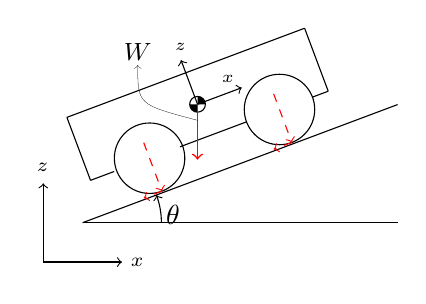
\begin{tikzpicture}
			\draw[->] (0.0, 0.0) -- (1.0, 0.0) node[pos=1.2] {$\WorldFrame_x$};
			\draw[->] (0.0, 0.0) -- (0.0, 1.0) node[pos=1.2] {$\WorldFrame_z$};
			\draw (0.5, 0.5) -- (4.5, 0.5);
			\draw (0.5, 0.5) -- (4.5, 2.0);
			\draw[->] (1.5, 0.5) arc [start angle=0, end angle=20.55604522, x radius = 1.0, y radius = 1.0] node[black, below right] {$\theta$};
			\draw (1.35, 1.31875) circle (0.4472135955cm);
			\draw (3.0, 1.9375) circle (0.4472135955cm);
			\draw (0.6, 1.0375) -- (0.9000108619, 1.150004073);
			\draw (1.737489138, 1.464058427) -- (2.581260862, 1.780472823);
			\draw (3.418739138, 2.094527177) -- ( 3.618739138, 2.169527177);
			\draw (0.6, 1.0375) -- (0.3, 1.837500002);
			\draw ( 3.618739138, 2.169527177) -- ( 3.318739138, 2.969517176);
			\draw ( 3.318739138, 2.969517176) -- (0.3, 1.837500002);
			
			\fill (1.959369569, 2.003513589) -- ++(0.1cm, 0) arc [start angle = 0, end angle = 90, x radius = 0.1, y radius = 0.1] -- ++(0, -0.2cm) arc [start angle = 270, end angle = 180, x radius = 0.1, y radius = 0.1 ];
        	\draw (1.959369569, 2.003513589) circle (0.1cm);
        	
        	\draw[->, red, line width = 0.2mm] (1.959369569, 2.003513589) -- (1.959369569, 1.3);
        	
        	\draw[dashed, ->, red] ( 1.507027977, 0.9000108619 ) -- ( 1.275735838, 0.8132763098 );
        	\draw[dashed, ->, red] ( 1.275735838, 1.516789899 ) -- ( 1.507027977, 0.9000108619 );
        	
        	\draw[dashed, ->, red] ( 3.157027177, 1.518760862 ) -- ( 2.925735038, 1.43202631 );
        	\draw[dashed, ->, red] ( 2.925735038, 2.135539899 ) -- ( 3.157027177, 1.518760862 );
        	
        	\draw[->] (1.959369569, 2.003513589) -- ( 2.521167076, 2.214187654) node[above, pos = 0.7] {\footnotesize $\BodyFrame_x$};
        	\draw[->] (1.959369569, 2.003513589) -- (1.748695504, 2.565311096)node[above] {\footnotesize $\BodyFrame_z$};
        	
        	\draw[->, line width=0.1pt] ( 1.959369569, 1.8 ) .. controls (1.2, 2.0) .. ( 1.2, 2.5 ) node[pos=1.1] {\small $W$};
        	
        	%\draw[->, line width=0.1pt] (3.05, 1.45) .. controls(3.05, 1.2) .. (2.85, 0.95) node[pos=1.1] {\tiny $\frac{W}{4} \sin(\theta)$};
        	
        %	\draw[->, line width=0.1pt] (3.1, 1.8) .. controls(3.6, 1.8) .. (3.6, 1.4) node[pos=1.1] {\tiny $\frac{W}{4} \cos(\theta)$};
			
		\end{tikzpicture}
	}
	\subfigure[Weight distribution during roll.] {
		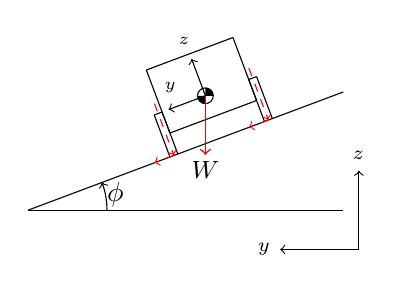
\begin{tikzpicture}
			\draw[->] (4.7, 0.0) -- (3.7, 0.0) node[pos=1.2] {$\WorldFrame_y$};
			\draw[->] (4.7, 0.0) -- (4.7, 1.0) node[pos=1.2] {$\WorldFrame_z$};
			
			\draw (0.5, 0.5) -- (4.5, 0.5);
			\draw (0.5, 0.5) -- (4.5, 2.0);
			\draw[->] (1.5, 0.5) arc [start angle=0, end angle=20.55604522, x radius = 1.0, y radius = 1.0] node[black, below right,pos = 1.4] {$\phi$};
			
			\draw (2.3, 1.175) -- (2.1, 1.708333333);
			\draw (2.4, 1.2125) -- ( 2.2, 1.745833333);
			\draw (2.1, 1.708333333) -- ( 2.2, 1.745833333); 
			
			\draw (3.5, 1.625) -- (3.3, 2.1583333);
			\draw (3.6, 1.6625) -- (3.4, 2.19583333);
			\draw (3.3, 2.1583333) -- (3.4, 2.19583333);
			
			\draw (2.3, 1.47916666) -- ( 3.4, 1.89166666 );
			
			\draw (2.3, 1.47916666) -- (2.0, 2.279166666);
			
			\draw ( 3.4, 1.89166666 ) -- (3.1, 2.691666634);
			
			\draw (2.0, 2.279166666) -- (3.1, 2.691666634);
			
			\fill (2.75, 1.9520833 ) -- ++(0.1cm, 0) arc [start angle = 0, end angle = 90, x radius = 0.1, y radius = 0.1] -- ++(0, -0.2cm) arc [start angle = 270, end angle = 180, x radius = 0.1, y radius = 0.1 ];
        	\draw (2.75, 1.9520833 ) circle (0.1cm);
        	
        	\draw[red, ->, line width = 0.2mm] (2.75, 1.9520833 ) -- (2.75, 1.2) node[black, pos=1.25] {\small $W$};		
        	\draw[dashed, red, ->] (2.35, 1.19375) -- (2.102739737, 1.101027401);
        	\draw[dashed, red, ->] (2.102739737, 1.853110701) -- (2.35, 1.19375);
			
			\draw[dashed, red, ->] (3.55, 1.64375) -- (3.302739737, 1.551027401);	
			\draw[dashed, red, ->] (3.302739737, 2.303110701) -- (3.55, 1.64375);	
			
			\draw[->] (2.75, 1.9520833 ) -- (2.574438279, 2.420247889) node[pos = 1.5] {\footnotesize $\BodyFrame_z$};
			\draw[->] (2.75, 1.9520833 ) -- (2.281835411, 1.776521579) node[ above left, pos = 0.5] {\footnotesize $\BodyFrame_y$};
			
			%\draw[->, line width=0.1pt]  (3.45, 1.58) -- (3.45, 1.3) node[pos=1.4] {\tiny $\frac{W}{4} \sin(\phi)$};
			%\draw[->, line width=0.1pt]  (2.102739737, 1.853110701) .. controls (2.0, 1.95) and (2.1, 1.7) .. (1.9, 1.7) node[pos=1.4] {\tiny $\frac{W}{4} \cos(\phi)$};
			
		\end{tikzpicture}
	}
	\caption{Forces and moments distribution.}
    \label{fig:wheelForcesMoments}
\end{figure}

Each wheel joint can only be actuated around the wheel horizontal axis, which is parallel to $\BodyFrame_y$. Every wheel holds a frame $\BodyFrame^i$ parallel to $\BodyFrame$, centered at its \acrshort{com}. Then, it also holds a frame $\WheelFrame^i$ which follows up the wheel velocity vector (section \ref{subsection:contactAngles}). Apart from it, each wheel is subject to forces and moments coming from its interaction with the terrain or due to gravity (figure \ref{fig:wheelForcesMoments}). Finally, these forces and moments shall be expressed with respect to frame $\BodyFrame$ and summed up in order to return a dynamics relationship of the mobile robot (equation \ref{eq:dynamics}).

The weight distribution on the mobile robot wheels is influenced by its roll and pitch. A dynamics model is derived based on Newton's second law as well as on the angular momentum rate of change from each wheel around its respective \acrshort{com}. The angular momentum rate of change of the whole mobile robot around its \acrshort{com} is also considered.

\begin{equation}
	\begin{aligned}
		\Mass \mathbf{\dot{\LinVelocity}} + \Mass \; \bm{\AngVelocity} \times \mathbf{\LinVelocity} &= \mathbf{\Force} \\
		\mathbf{\InertiaTensor} \bm{ \dot{\AngVelocity} } + \bm{\AngVelocity} \times (\mathbf{\InertiaTensor} \bm{\AngVelocity}) &= \sum_{i} \mathbf{\Moment}
	\end{aligned}	
	\label{eq:dynamics}
\end{equation}

, where $\Mass$ stands for the mobile robot mass. Moreover, $\mathbf{\InertiaTensor}$ denotes the inertia tensor of the mobile robot with respect to frame $\BodyFrame$. Furthermore, $\mathbf{\Force} = [f_x \; f_y \; f_z]^T$ stands for the sum of forces acting on the system and $\mathbf{\Moment} = [\mx \; \my \; \mz]^T$ denotes the sum of moments. $\mathbf{\Force}$ and $\mathbf{\Moment}$ are expressed with respect to frame $\BodyFrame$. 

Equation \ref{eq:dynamics} may be obtained by applying the second newton law for translational and rotational dynamics. It is of interest to find out a dynamics formulation which is expressed with respect to $\BodyFrame$, because $\mathbf{\InertiaTensor}$ is constant but also because it is more intuitive to think of velocities, forces and moments with respect to $\BodyFrame$. In case the linear and angular moments are defined by $\mathbf{\linearMoment} = \Mass \mathbf{\LinVelocity}$ and $\mathbf{\angularMoment} = \mathbf{\InertiaTensor} \bm{\AngVelocity}$ respectively, it is possible to derive a dynamics formulation with the help of equation \ref{eq:vectorDiff2}. From now on, for the sake of completeness, each moment and force acting on the mobile robot are presented.

%%%%%%%%%%%%%%%%%%%%%%%%%%%%%%%%%%%%%%%%%%%%%%%%%%%%%%%%%%%%%%%%%%%%%%%%
\subsection{Wheel actuation}
\label{subsection:wheelActuation}

Every wheel is commanded by a torque, $\bm{\Torque}_i$, which is computed by a control loop at every iteration. $\bm{\Torque}_i$ is expressed with respect to $\BodyFrame$ and it only holds a lateral component in that frame. That torque yields a traction force $\mathbf{\Traction}_i$ which is expressed with respect to the wheel frame $\WheelFrame^i$ (figure \ref{fig:wheelForcesMoments}). The traction force $\mathbf{\Traction}_i$ only holds a single longitudinal component within $\WheelFrame^i$. $\mathbf{\Traction}_i$ is the result of the action of the soil on the wheel at $\contactPoint_i$. Therefore, the force produced by $\bm{\Torque}_i$ on the soil opposes $\mathbf{\Traction}_i$. The wheel frame $\WheelFrame^i$ is centered at the wheel center and follows up the wheel velocity vector, which may not match frame $\BodyFrame^i$. Finally, it comes that,

\begin{equation}
	\bm{\Torque}_i = -\mathbf{\wheelToContact}_i \times \Bigl( \mathbf{\RotMatrix}_{\WheelFrame^i}^{\BodyFrame} \mathbf{\Traction}_i \Bigr), \; i = 1, ..., 4
	\label{eq:actuatedForce}
\end{equation}

, where $\mathbf{\wheelToContact}_i$ stands for a vector which connects each wheel center to $\contactPoint_i$, with respect to $\BodyFrame$. Therefore, in order to determine the total force and moment produced by wheel actuation, one needs to express every traction force $\mathbf{\Traction}_i$ with respect to $\BodyFrame$, by taking into account equation \ref{eq:rotationMatrixB2T}. Then, the sum of traction forces, $\mathbf{\Traction}$, with respect to $\BodyFrame$ are expressed as,

\begin{equation}
	\mathbf{\Traction} = \sum_{i = 1}^{4} \mathbf{\RotMatrix}_{\WheelFrame^i}^{\BodyFrame} \mathbf{\Traction}_i
	\label{eq:totalActuatedForce}
\end{equation}

The traction forces produced by wheel torque actuation may also output a moment around \acrshort{com} with respect to $\BodyFrame$.

\begin{equation}
	\mathbf{\Moment}_{\mathbf{\Traction}} = \sum_{i = 1}^{4} \mathbf{\contactPoint}_i \times \Bigl( \mathbf{\RotMatrix}_{\WheelFrame^i}^{\BodyFrame} \mathbf{\Traction}_i \Bigr) + \bm{\Torque}_i
	\label{eq:totalActuatedMoment}
\end{equation}

, where $\mathbf{\contactPoint}_i$ is a vector connecting the mobile robot \acrshort{com} to the contact point $\contactPoint_i$, with respect to $\BodyFrame$. From this definition, it is worth noticing that $\mathbf{\wheelPosition}_i + \mathbf{\wheelToContact}_i = \mathbf{\contactPoint}_i$. From this result it is possible to rewrite equation \ref{eq:totalActuatedMoment}, by taking equation \ref{eq:actuatedForce} into account.

\begin{equation}
	\mathbf{\Moment}_{\mathbf{\Traction}} = \sum_{i = 1}^{4} \mathbf{\wheelPosition}_i \times \left( \mathbf{\RotMatrix}_{\WheelFrame^i}^{\BodyFrame} \mathbf{\Traction}_i \right)
	\label{eq:totalActuatedMomentSimple}
\end{equation}

If equations \ref{eq:totalActuatedMomentSimple} nd \ref{eq:totalActuatedForce} are combined with equation \ref{eq:actuatedForce}, it comes that,

\begin{equation}
	\bm{\Torque} = -\sum_{i = 1}^{4} \mathbf{\SkewSymmetricMatrix}(\mathbf{\wheelToContact}_i) \mathbf{\Traction}_i \quad \mathbf{\Moment}_{\mathbf{\Traction}} = -\sum_{i = 1}^{4} \mathbf{\SkewSymmetricMatrix}(\mathbf{\wheelPosition}_i) \mathbf{\Traction}_i
	\label{eq:tractionMomentTorque}
\end{equation}

\subsection{Wheel spin rate}
\label{subsection:wheelSpinRate}

Each wheel is considered to spin only if a torque $\bm{\Torque}_i$ is fed to the wheel along its lateral axis. In case no torque is available, the wheel spin rate, $\mathbf{\dot{\wheelAngPosition}}_i$, is considered to be zero.

\begin{equation}	
	\mathbf{\InertiaTensor}_{\text{wheel}} \mathbf{\ddot{\wheelAngPosition}}_i = \bm{\Torque}_i
	\label{eq:wheelSpinRate}
\end{equation}

The variables introduced into equation \ref{eq:wheelSpinRate} are expressed with respect to $\BodyFrame$. Then, $\mathbf{\wheelAngPosition}_i = [0, \wheelAngPosition_i, 0]^T$ and $\mathbf{\wheelAngPosition} = [\mathbf{\wheelAngPosition}_1^T, \mathbf{\wheelAngPosition}_2^T, \mathbf{\wheelAngPosition}_3^T, \mathbf{\wheelAngPosition}_4^T]^T$.

\begin{assumption}
	If a torque is not fed to wheel $i$, its spin rate  is zero.
	\label{assumption:velTzNeglected}
\end{assumption}

%%%%%%%%%%%%%%%%%%%%%%%%%%%%%%%%%%%%%%%%%%%%%%%%%%%%%%%%%%%%%%%%%%%%%%%%
\subsection{Wheel-terrain contact model}
\label{subsection:wheelTerrainContactModel}

The ability to accurately model the interaction forces and moments between a wheel and the contact terrain is of the utmost importance, in order to simulate a theoretical model of a robot or to control a real-life application at a given environment.

There are four possible cases of wheel-terrain interaction (figure \ref{fig:contactModels}): rigid wheel on rigid terrain, rigid wheel on deformable terrain, deformable wheel on rigid terrain and a deformable wheel on deformable terrain. In references \cite{Genta2012, Yoshida2016}, one can find analytical models for all these possibilities.

\begin{figure}[!htb]
  \centering
  \begin{subfigmatrix}{4}
  	\subfigure[Rigid wheel contacting with rigid terrain]{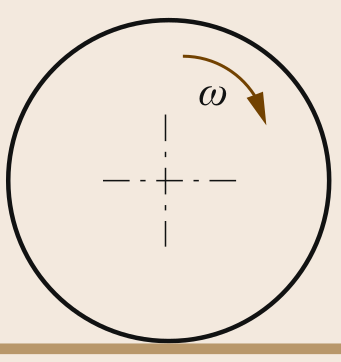
\includegraphics[width=0.15\linewidth]{Figures/rigid_rigid.png}}
    \subfigure[Rigid wheel contacting with deformable terrain]{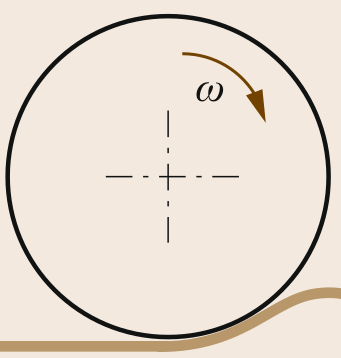
\includegraphics[width=0.15\linewidth]{Figures/rigid_deformable.png}}
    \subfigure[Deformable wheel contacting with rigid terrain]{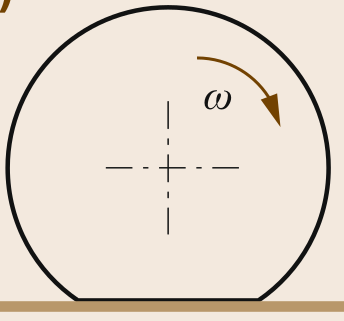
\includegraphics[width=0.15\linewidth]{Figures/deformable_rigid.png}}
    \subfigure[Deformable wheel contacting with deformable terrain]{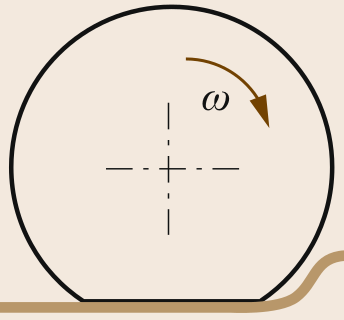
\includegraphics[width=0.15\linewidth]{Figures/deformable_deformable.png}}
  \end{subfigmatrix}
  \caption{Wheel-terrain contact models \cite{Yoshida2016}}
  \label{fig:contactModels}
\end{figure}

In this thesis, only rigid wheels are considered. Even if a wheel presents some degree of deformability (i.e. pneumatic tire), it can be modeled as a rigid wheel if the average tire ground pressure is higher than the critical ground pressure, $p_{gcr}$.

\begin{equation}
	p_{gcr} = \Biggl(\frac{k_c}{b} + k_{\phi}\Biggr)^{\frac{1}{2n+1}} \, \Biggl(\frac{3W}{(3-n)b_{ti}\sqrt{D}} \Biggr)^{\frac{2n}{2n+1}}
\end{equation}

When it comes to the type of soil, a rover may traverse deformable (sand) or rigid terrain (rock) when it is deployed at a realistic planetary environment, so it is difficult to predict \textit{a priori} what kind of soil it will be traversing as well as its properties.

The theory of terramechanics focuses on studying the mechanical properties of soils and to assess its behaviour, when it is subject to the influence of a robot with a locomotion set. Apart from it, terramechanics models also deliver performance quantification by describing the stress fields that the contact modules are exposed to. In case of deformable soils, the standard model descriptor is the Bekker-Wong model. On the other hand, the Coulomb friction model fits well to describe the contact between rigid wheels and rigid terrain.

In this thesis, deformable terrain contact physics is discarded as a simulation option because the physics engine of Gazebo, \acrshort{ode}, does not provide a test-bed for it, but also due to the fact that it is cumbersome to online estimate the parameters of deformable terrain. There are open-source terramechanics real-time simulators (Project Chrono, Vortex) which could enable the simulation of deformable terrain, however these simulators do not provide a bridge to ROS, which is used as a message transmission mechanism between nodes to exchange data among multiple parallel processes. The Coulomb friction model is implemented within \acrshort{ode} to match as close as possible the contact physics between rigid objects.

\subsubsection{Coulomb friction model}
\label{subsubsection:coulombFrictionModel}

This model provides a friction force, $\mathbf{\ForceSubscript{\FrictionSubscript}}$, acting at each wheel, as a result of the action of the soil on the wheel. This forces acts at $\contactPoint_i$ with a direction opposite to the wheel velocity $\mathbf{\LinVelocity}_i$. $\mathbf{\ForceSubscript{\FrictionSubscript}}$ breaks into a longitudinal ($\ForceSubscriptTwo{\FrictionSubscript}{x}$) and lateral ($\ForceSubscriptTwo{\FrictionSubscript}{y}$) component, in case $\ForceSubscript{\FrictionSubscript}$ is expressed with respect to $\WheelFrame^i$. Apart from this, a terrain reaction force $\mathbf{\ForceSubscript{\NormalForceSubscript}}$, acts at $\contactPoint_i$, with a direction parallel to the contact normal at $\contactPoint_i$, so $\mathbf{\ForceSubscript{\NormalForceSubscript}}$ only holds a single vertical component within $\WheelFrame^i$. The Coulomb friction model states the following,

\begin{equation}
	\begin{cases}
		\left(\frac{\ForceSubscriptTwo{\FrictionSubscript}{x}}{\FrictionCoefficient_x \ForceSubscript{\NormalForceSubscript}} \right)_i^2 + \left( \frac{\ForceSubscriptTwo{\FrictionSubscript}{y}}{\FrictionCoefficient_y \ForceSubscript{\NormalForceSubscript}} \right)_i^2 \leq 1\\
		\left( \ForceSubscript{\NormalForceSubscript} \right)_i > 0
	\end{cases}, \; i = 1, ..., 4
	\label{eq:coulombFrictionModel}
\end{equation}

Equation \ref{eq:coulombFrictionModel} states that $\left( \mathbf{\ForceSubscript{\FrictionSubscript}} \right)_i$ lies within an ellipse with diagonals $\FrictionCoefficient_x \left( \ForceSubscript{\NormalForceSubscript} \right)_i$ and $\FrictionCoefficient_y \left( \ForceSubscript{\NormalForceSubscript} \right)_i$. In case $\FrictionCoefficient_x = \FrictionCoefficient_y$, the ellipse turns into a circle. $\FrictionCoefficient_x$ and $\FrictionCoefficient_y$ denote friction coefficients along the longitudinal and lateral components of $\WheelFrame^i$, respectively.

If a wheel $i$ sticks to the contact point $\contactPoint_i$, it means equation \ref{eq:coulombFrictionModel} is smaller than one. On the other hand, if a wheel is sliding, equation \ref{eq:coulombFrictionModel} equals one and $\left( \mathbf{\ForceSubscript{\FrictionSubscript}} \right)_i$ has an opposite direction to $\left( \mathbf{\LinVelocity}_i \right)_{\WheelFrame^i}$. In case wheel $i$ is not subject to a traction force at $\contactPoint_i$ and holds a null linear velocity, it is assumed that $\left( \mathbf{\ForceSubscript{\FrictionSubscript}} \right)_i = \mathbf{0}$. 

\begin{equation}
	\begin{cases}
		\left( \mathbf{\ForceSubscript{\FrictionSubscript}} \right)_i = -( \mathbf{\Traction}_i + \mathbf{\gravity}_i), \; \mathbf{\LinVelocity}_i = \mathbf{0} \wedge \mathbf{\LinAccel}_i = \mathbf{0} \\ \vspace{2mm}
		\left( \mathbf{\ForceSubscript{\FrictionSubscript}} \right)_i = -\left\Vert \left( \FrictionCoefficient_x \ForceSubscript{\NormalForceSubscript} \sqrt{1 - \left( \frac{\ForceSubscriptTwo{\FrictionSubscript}{y}}{\FrictionCoefficient_y \ForceSubscript{\NormalForceSubscript}}  \right)^2 }; \ForceSubscriptTwo{\FrictionSubscript}{y}; 0 \right) \right\Vert \cdot \left( \frac{\mathbf{\LinVelocity}_i}{ \| \mathbf{\LinVelocity}_i \| } \right)_{\WheelFrame^i}, \; \mathbf{\LinVelocity}_i \neq \mathbf{0} \\ \vspace{2mm}
		\left( \mathbf{\ForceSubscript{\FrictionSubscript}} \right)_i = -\left\Vert \left( \FrictionCoefficient_x \ForceSubscript{\NormalForceSubscript} \sqrt{1 - \left( \frac{\ForceSubscriptTwo{\FrictionSubscript}{y}}{\FrictionCoefficient_y \ForceSubscript{\NormalForceSubscript}}  \right)^2 }; \ForceSubscriptTwo{\FrictionSubscript}{y}; 0 \right) \right\Vert \cdot \left( \frac{\mathbf{\LinAccel}_i}{ \| \mathbf{\LinAccel}_i \| } \right)_{\WheelFrame^i}, \; \mathbf{\LinVelocity}_i = \mathbf{0} \wedge \mathbf{\LinAccel}_i \neq \mathbf{0}
	\end{cases}
	\label{eq:friction}
\end{equation}

\begin{assumption}
	If the torque fed to wheel $i$ and its linear velocity are zero, the friction force of wheel $i$ acting at $\contactPoint_i$ is considered to be zero.	
\end{assumption}

The sum of friction forces $\mathbf{\ForceSubscript{\FrictionSubscript}}$ acting on the mobile robot and the yielded sum of moments are given by,

\begin{equation}
	\mathbf{\ForceSubscript{\FrictionSubscript}} = \sum_{i=1}^{4} \mathbf{\RotMatrix}_{\WheelFrame^i}^{\BodyFrame} \left( \mathbf{\ForceSubscript{\FrictionSubscript}} \right)_i \quad \mathbf{\Moment}_{\left( \mathbf{\ForceSubscript{\FrictionSubscript}} \right)} = \sum_{i = 1}^{4} \mathbf{\SkewSymmetricMatrix}(\mathbf{\contactPoint}_i) \mathbf{\RotMatrix}_{\WheelFrame^i}^{\BodyFrame} \left( \mathbf{\ForceSubscript{\FrictionSubscript}} \right)_i
	\label{eq:frictionMomentForce}
\end{equation}

Finally, the determination of $\left( \mathbf{\ForceSubscript{\NormalForceSubscript}} \right)_i$ is made by computing the portion of the mobile robot weight every wheel $i$ supports, which is presented in \ref{subsubsection:effectsGravity}.

\subsubsection{Effects of gravity}
\label{subsubsection:effectsGravity}

Gravity pushes the mobile robot into the terrain. As a response, ground reaction forces $\left( \mathbf{\ForceSubscript{\NormalForceSubscript}} \right)_i$ sustain the mobile robot, by avoiding terrain failure. At each wheel $i$, the effect of gravity acting at $\contactPoint_i$ is denoted by $\left( \mathbf{\ForceSubscript{\gravity}} \right)_i$, which is expressed with respect to $\WheelFrame^i$. The vertical component of $\left( \mathbf{\ForceSubscript{\gravity}} \right)_i$ equals $\left( \mathbf{\ForceSubscript{\NormalForceSubscript}} \right)_i$ and are orthogonal to $\left( \mathbf{\ForceSubscript{\FrictionSubscript}} \right)_i$  and $\mathbf{\Traction}_i$. The sum of $\left( \mathbf{\ForceSubscript{\gravity}} \right)_i$ for every wheel equals the mobile robot weight.

\begin{equation}
	\Mass \mathbf{\gravity} = \mathbf{\RotMatrix}_{\BodyFrame}^{\WorldFrame} \sum_{i=1}^{4} \mathbf{\RotMatrix}_{\WheelFrame^i}^{\BodyFrame} \left( \mathbf{\ForceSubscript{\gravity}} \right)_i \quad , \quad \left( \ForceSubscriptTwo{\gravity}{z} \right)_i = - \left( \ForceSubscriptTwo{\NormalForceSubscript}{z} \right)_i
	\label{eq:gravitySum}
\end{equation}

, where $\mathbf{\gravity}$ denotes the gravity vector with respect to $\WorldFrame$. The sum of the effects of gravity and ground reaction forces are stated by,

\begin{equation}
	\mathbf{\ForceSubscript{\gravity}} = \sum_{i=1}^{4} \mathbf{\RotMatrix}_{\WheelFrame^i}^{\BodyFrame} \left( \mathbf{\ForceSubscript{\gravity}} \right)_i \quad \mathbf{\ForceSubscript{\NormalForceSubscript}} = \sum_{i=1}^{4} \mathbf{\RotMatrix}_{\WheelFrame^i}^{\BodyFrame} \left( \mathbf{\ForceSubscript{\NormalForceSubscript}} \right)_i
	\label{eq:sumGravityReaction}
\end{equation}

The sum of moments created by all ground reaction forces around the mobile robot \acrshort{com} is denoted by $\mathbf{\Moment}_{\left( \mathbf{\ForceSubscript{\NormalForceSubscript}} \right)}$. Likewise, the sum of moments created by the effect of gravity on every wheel is denoted by $\mathbf{\Moment}_{\left( \mathbf{\ForceSubscript{\gravity}} \right)}$ and equals zero.

\begin{equation}
	\mathbf{\Moment}_{\left( \mathbf{\ForceSubscript{\NormalForceSubscript}} \right)} = \sum_{i=1}^{4} \mathbf{\contactPoint}_i \times \left( \mathbf{\RotMatrix}_{\WheelFrame^i}^{\BodyFrame} \left( \mathbf{\ForceSubscript{\NormalForceSubscript}} \right)_i \right) = \mathbf{0} \quad \mathbf{\Moment}_{\left( \mathbf{\ForceSubscript{\gravity}} \right)} = \sum_{i=1}^{4} \mathbf{\contactPoint}_i \times \left( \mathbf{\RotMatrix}_{\WheelFrame^i}^{\BodyFrame} \left( \mathbf{\ForceSubscript{\gravity}} \right)_i \right) = \mathbf{0}
	\label{eq:groundReactionForcesMoment}
\end{equation}

%%%%%%%%%%%%%%%%%%%%%%%%%%%%%%%%%%%%%%%%%%%%%%%%%%%%%%%%%%%%%%%%%%%%%%%%
\section{Slippage}
\label{section:slippage}

During the traversal of a planetary environment, a wheeled mobile robot may experience slip at each wheel $i$, both on the longitudinal ($\SlipRatio_i$) and lateral ($\SlipAngle_i$) directions of the wheel frame $\WheelFrame_i$, where $\SlipRatio_i$ stands for the slip ratio at wheel $i$ and $\SlipAngle_i$ denotes the slip angle at wheel $i$. Although the slip angle $\SlipAngle_i$ may be measured at each wheel frame $\WheelFrame_i$, it is more usual to do it in case of steering wheels. Instead, the slip angle is computed with the mobile robot \acrshort{com} velocities within frame $\BodyFrame$, due to the fact that 

\begin{equation}
  	\begin{aligned}
      		\SlipRatio_i = \begin{cases}
						1 - \frac{ \left( \vx_i \right)_{\WheelFrame^i}}{\WheelRadius \; \dot{\wheelAngPosition}_i}, \quad \text{if} \quad |\WheelRadius \; \dot{\wheelAngPosition}_i| \geq | \left( \vx_i \right)_{\WheelFrame^i}| \; \text{(slip)}\\
						\frac{\WheelRadius \; \dot{\wheelAngPosition}_i}{\left( \vx_i \right)_{\WheelFrame^i}} - 1, \quad \text{if} \quad |\WheelRadius \; \dot{\wheelAngPosition}_i| < | \left( \vx_i \right)_{\WheelFrame^i}| \; \text{(skid)}
							\end{cases}
    	\end{aligned} \qquad
    	\begin{aligned}
      		\SlipAngle = \begin{cases}
							\arctan{\left( \frac{\vy}{\vx} \right)}, \quad (\vx \neq 0)\\
							\text{sgn}(\vy) \cdot \frac{\pi}{2} \quad (\vx = 0)
						\end{cases}
    	\end{aligned}
    	\label{eq:slip}
\end{equation}

, where $\WheelRadius$ denotes the wheel radius. Physical parameters related to every wheel are equal. If $0 \leq \SlipRatio_i \leq 1$, it is said wheel $i$ is slipping. If $-1 \leq \SlipRatio_i < 0$, it is said that wheel $i$ is skidding or braking. However, if the signs of $\left( \vx_i \right)_{\WheelFrame^i}$ and $\dot{\wheelAngPosition}_i$ are opposite to each other, it means $1 < |\SlipRatio_i| \leq 2$. Although these impractical slips are possible \cite{Peiret2021}, no terramechanics analytical models are presented, because no literature was found with research on the topic. Regarding the slip angle $\SlipAngle$, this quantity is as high as the lateral skid, $\vy$, is with respect to the longitudinal velocity, $\vx$.

In accordance to the definitions presented above, it is possible to define a new quantity, $\surfaceRelVel_i$, which expresses the relative velocity between wheel $i$ at $\contactPoint_i$ and the surface.

\begin{equation}
	\delta_i = r \dot{\wheelAngPosition}_i - \left( \vx_i \right)_{\WheelFrame^i}
	\label{eq:relativeVelocity}
\end{equation}

, with $\bm{\delta} = [\delta_1, \delta_2, \delta_3, \delta_4]^T$. In case $\delta_i = 0$, wheel $i$ presents a pure rolling motion. Apart from that, wheel $i$ exhibits a slipping or skidding behaviour.

\section{Full state-space model}
\label{section:fullStateSpace}

In order to sum up the previous sections, it is possible to deliver a full state-space model with respect to the state vector $[\mathbf{\Position}^T \; \bm{\Orientation}^T \; \mathbf{\LinVelocity}^T \; \bm{\AngVelocity}^T \; \mathbf{\dot{\wheelAngPosition}}^T]^T$.

\begin{equation}
	\begin{cases}
		\DerMathBold{\Position} = \mathbf{\RotMatrix}_{\BodyFrame}^{\WorldFrame} (\yaw, \pitch, \roll) \mathbf{\LinVelocity}\\
		\DerBold{\Orientation} = \mathbf{\bar{\RotMatrix}}_{\BodyFrame}^{\WorldFrame} (\yaw, \pitch, \roll) \bm{\AngVelocity}\\
		\mathbf{\dot{\LinVelocity}} = -\bm{\AngVelocity} \times \mathbf{\LinVelocity} + \frac{1}{\Mass} \mathbf{\Force}\\
		\bm{ \dot{\AngVelocity} } = \mathbf{\InertiaTensor}^{-1} \left( -\bm{\AngVelocity} \times \left( \mathbf{\InertiaTensor} \bm{\AngVelocity} \right) + \mathbf{\Moment} \right)\\
		\mathbf{\ddot{\wheelAngPosition}}_i = \mathbf{\InertiaTensor}_{\text{wheel}}^{-1} \bm{\Torque}_i 
	\end{cases}
	\label{eq:fullStateSpace}
\end{equation}

According to equations \ref{eq:tractionMomentTorque}, \ref{eq:frictionMomentForce}, \ref{eq:sumGravityReaction}, the total sum of forces acting on the mobile robot around \acrshort{com} with respect to $\BodyFrame$, is expressed as follows,

\begin{equation}
	\mathbf{\Force} = \mathbf{\ForceSubscript{\gravity}} + \mathbf{\ForceSubscript{\NormalForceSubscript}} + \mathbf{\ForceSubscript{\FrictionSubscript}} + \mathbf{\Traction} = \sum_{i=1}^{4} \mathbf{\RotMatrix}_{\WheelFrame^i}^{\BodyFrame} \left[ \left( \mathbf{\ForceSubscript{\gravity}} \right)_i + \left( \mathbf{\ForceSubscript{\NormalForceSubscript}} \right)_i + \left( \mathbf{\ForceSubscript{\FrictionSubscript}} \right)_i + \mathbf{\Traction}_i \right]
	\label{eq:sumForcesBody}
\end{equation}

If one also takes into account equation \ref{eq:groundReactionForcesMoment}, the total sum of moments acting on the mobile robot around \acrshort{com} is given by equation \ref{eq:sumMomentsBody}. Every cross product is replaced by a skew symmetric matrix (see section \ref{section:skewSymmetricMatrix}). 

\begin{equation}
	\mathbf{\Moment} = \mathbf{\Moment}_{\mathbf{\Traction}} + \mathbf{\Moment}_{\left( \mathbf{\ForceSubscript{\NormalForceSubscript}} \right)} + \mathbf{\Moment}_{\left( \mathbf{\ForceSubscript{\gravity}} \right)} + \mathbf{\Moment}_{\left( \mathbf{\ForceSubscript{\FrictionSubscript}} \right)} = \sum_{i=1}^{4} \mathbf{\SkewSymmetricMatrix}(\mathbf{\contactPoint}_i) \mathbf{\RotMatrix}_{\WheelFrame^i}^{\BodyFrame} \left[ \left( \mathbf{\ForceSubscript{\gravity}} \right)_i + \left( \mathbf{\ForceSubscript{\NormalForceSubscript}} \right)_i + \left( \mathbf{\ForceSubscript{\FrictionSubscript}} \right)_i \right] - \mathbf{\SkewSymmetricMatrix}(\mathbf{\wheelPosition}_i) \mathbf{\Traction}_i
	\label{eq:sumMomentsBody}
\end{equation}

, where $\mathbf{x} = [\mathbf{\Position}^T, \bm{\Orientation}^T, \mathbf{\LinVelocity}^T, \bm{\AngVelocity}^T, \mathbf{\wheelAngPosition}^T]^T$, $\mathbf{z} = [ \mathbf{\Force}^T, \mathbf{\Moment}^T, \mathbf{\LinVelocity}_i^T, \SlipRatio_i, \SlipAngle_i, \SlipAngle]^T$, $\mathbf{p} = [\FrictionCoefficient, \WheelRadius, \mathbf{\contactPoint}_i^T, \mathbf{\gravity}^T, {\InertiaTensor}_{yy, \text{wheel}}, {\InertiaTensor}_{ij}]^T$.